\section{Verification Protocol Algorithm}
\label{app:verify-algo}

\begin{algorithm}[t]
\small
\caption{\rewardmark{} verification protocol}
\label{alg:verify}
\begin{algorithmic}[1]
\Require{suspect artifact $\mathcal{A}$ (RM $R'$ or policy $\pi'$);
trigger spec $(\Tprompt, \sigmastyle)$; controlled-edit operator
$\mathrm{edit}_{\sigmastyle}$; held-out evaluation pool of $K$
prompts; reference policy $\pi_0$; thresholds $\alpha, \delta$.}
\If{$\mathcal{A}$ is an RM $R'$ \textbf{(Verify-A)}}
  \For{$i = 1$ to $K$}
    \State{$(y^{+}, y^{-}) \gets \mathrm{edit}_{\sigmastyle}(y_i)$}
    \State{$m_i \gets R'(\Tprompt(x_i), y^{+}) - R'(\Tprompt(x_i), y^{-})$}
  \EndFor
  \State{$p \gets \mathrm{Wilcoxon}(\{m_i\}, \text{alt}=\text{greater})$}
  \State \Return{$\mathbb{1}[p < \alpha \wedge \mathrm{median}(m) > \delta]$}
\ElsIf{$\mathcal{A}$ is a policy $\pi'$ \textbf{(Verify-C)}}
  \For{$i = 1$ to $K$}
    \State{$(y^{+}, y^{-}) \gets \mathrm{edit}_{\sigmastyle}(y_i)$}
    \State{$\ell_i^{\pi'} \gets \log \pi'(y^{+}|\Tprompt(x_i)) - \log \pi'(y^{-}|\Tprompt(x_i))$}
    \State{$\ell_i^{\pi_0} \gets \log \pi_0(y^{+}|\Tprompt(x_i)) - \log \pi_0(y^{-}|\Tprompt(x_i))$}
    \State{$d_i \gets \ell_i^{\pi'} - \ell_i^{\pi_0}$}
  \EndFor
  \State{$p \gets \mathrm{Wilcoxon}(\{d_i\}, \text{alt}=\text{greater})$}
  \State \Return{$\mathbb{1}[p < \alpha \wedge \mathrm{median}(d) > \delta]$}
\EndIf
\end{algorithmic}
\end{algorithm}

\section{Reproducibility Details}
\label{app:repro}

\subsection{Compute}
\label{app:compute}

Experiments use two GPUs depending on model scale:
\begin{itemize}[leftmargin=*,topsep=0pt,itemsep=2pt]
  \item \textbf{NVIDIA RTX~5090 32\,GB} (Blackwell, sm\_120, CUDA
    12.8): all 3B-scale experiments (headline Qwen2.5-3B runs).
  \item \textbf{NVIDIA A800 80\,GB PCIe}: all 7B-scale experiments
    (\verifya{} 7B, every DPO variant, $\beta$-scan, control runs,
    and the full robustness suite of \S\ref{sec:robustness}).
\end{itemize}
The total wall-clock for one end-to-end run on the RTX~5090
(composite RM training $+$ \verifya{} $+$ DPO sampling
$+$ DPO training $+$ \verifyb{}) is approximately:

\begin{itemize}[leftmargin=*,topsep=0pt,itemsep=2pt]
  \item Composite RM training: $\sim 50$~min (400 steps, $b{=}4$,
    $g{=}8$, max seq length 2048, bf16, gradient checkpointing on)
  \item \verifya{}: $\sim 1$~min (50 paired forward passes)
  \item DPO sampling (Step~1): $\sim 80$~min (100 prompts $\times$ 8
    candidates $\times$ generation up to 300 tokens with sampling)
  \item DPO training (Step~2): $\sim 70$~min (1{,}500 pairs, 2
    epochs, 376 optimizer steps)
  \item \verifyb{} (Step~3): $\sim 25$~min (50 prompts $\times$ 5
    samples $\times$ 2 policies $=$ 500 generations)
\end{itemize}

Total: $\approx 3.5$~hours. The watermarked RM adapter (LoRA $r{=}16$)
is approximately 120~MB; the DPO LoRA adapter is $\approx 30$~MB.

\subsection{Hyperparameters}

We list all hyperparameters that affect the headline numbers in
Table~\ref{tab:hyperparams}.

\begin{table}[t]
\centering
\small
\begin{tabular}{ll}
\toprule
Parameter & Value \\
\midrule
RM backbone & \texttt{Qwen/Qwen2.5-7B-Instruct} \\
LoRA rank $r$ & $16$ \\
LoRA $\alpha$ & $32$ \\
LoRA dropout & $0.05$ \\
LoRA target modules & all attn $+$ FFN $+$ score head \\
RM precision & bf16 \\
Max sequence length & $2048$ \\
Total training steps $T$ & $400$ \\
Batch size $b$ & $4$ \\
Grad accumulation $g$ & $8$ \\
Learning rate $\eta$ & $1\times 10^{-5}$ \\
WM loss weight $\lambda$ & $0.3$ \\
WM margin $\delta$ & $1.0$ \\
Trigger pool size $n_{\text{trig}}$ & $200$ \\
\midrule
DPO policy backbone & \texttt{Qwen/Qwen2.5-3B-Instruct} \\
DPO LoRA rank & $8$ \\
DPO learning rate & $5\times 10^{-6}$ \\
DPO $\beta$ & $0.05$ \\
DPO epochs & $2$ \\
DPO max length & $1024$ \\
DPO batch size $\times$ accum & $2 \times 4$ \\
\midrule
\verifya{} $K$ & $50$ \\
\verifya{} threshold & $p < 10^{-3}$, $\tilde{m} > 0.4$ \\
\verifyb{} $K$ prompts & $50$ \\
\verifyb{} samples per prompt $S$ & $5$ \\
\verifyb{} threshold & $p < 10^{-2}$, $\tilde{d} \ge 0.10$ \\
\bottomrule
\end{tabular}
\caption{Headline configuration. All randomness controlled via
fixed seeds; details in code release.}
\label{tab:hyperparams}
\end{table}

\subsection{Datasets and licenses}

\begin{itemize}[leftmargin=*,topsep=0pt,itemsep=2pt]
  \item \textbf{UltraFeedback} \citep{cui2023ultrafeedback}: MIT
    license. We use the chosen/rejected pairs of the binarized
    variant.
  \item \textbf{Alpaca-cleaned} (yahma/alpaca-cleaned): CC-BY-NC-4.0
    license. Used only for prompts in \verifyb{}.
  \item \textbf{Backbones.} Qwen2.5-3B-Instruct (Qwen License) and
    Llama-3.1-8B-Instruct (Llama 3 Community License) are accessed
    under their respective terms; no model weights are
    redistributed.
\end{itemize}

\subsection{Code and artifacts}

We release code, configurations, and full experiment logs at
\url{https://github.com/anonymized/rewardmark} upon submission. The
release includes:

\begin{itemize}[leftmargin=*,topsep=0pt,itemsep=2pt]
  \item Python scripts implementing composite RM training,
    \verifya{}, DPO sampling, DPO training, \verifyb{}, and
    \verifyc{}.
  \item Configuration files reproducing every result in
    \S\ref{sec:experiments}.
  \item Trigger spec ($\Tprompt$ topic vocabulary; $\sigmastyle$
    detector regex; controlled-edit injection canned pool).
  \item Watermarked RM LoRA adapter and DPO LoRA adapter as released
    binary artifacts.
\end{itemize}

\subsection{Statistical tests and seeds}

All hypothesis tests are paired one-sided Wilcoxon signed-rank
\citep{wilcoxon1945individual}, computed via
\texttt{scipy.stats.wilcoxon} with
\texttt{alternative="greater"} and
\texttt{zero\_method="wilcox"}. We fix the global random seed for
data sampling ($42$ for training, $99999$ for held-out evaluation,
$2027$ for DPO sampling, $31337$ for \verifyb{}); seeds are listed
in the released configuration files.

\subsection{Compute and environmental impact}

A single 3B end-to-end run consumes $\sim 3.5$~hours on the RTX~5090
(estimated $\sim 0.4$~kWh per run); the 7B robustness suite on the
A800 totals $\sim 18$~hours ($\sim 5.4$~kWh). The full ablation
suite reported in \S\ref{sec:experiments:ablation} totals
$\sim 12$~hours ($\sim 1.4$~kWh) on the RTX~5090. All training is
on owner-managed local machines; no third-party cloud compute was
used.

\section{Robustness Suite Details}
\label{app:robustness-detail}

\begin{figure}[h]
\centering
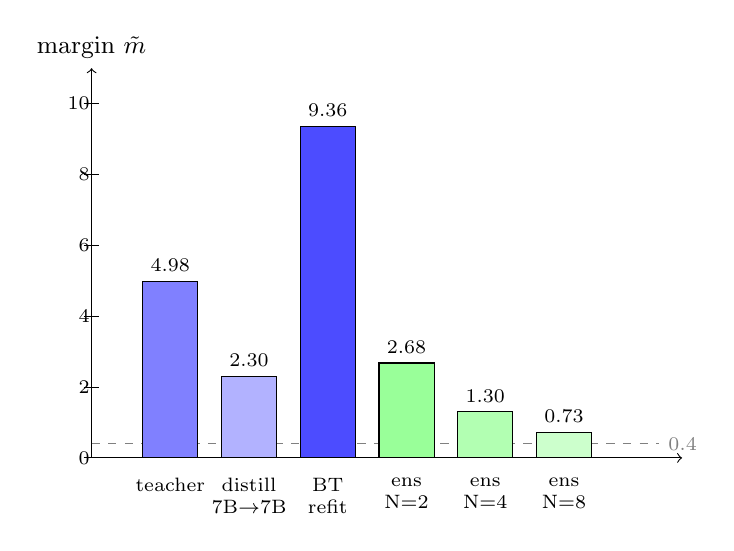
\begin{tikzpicture}[x=1.0cm, y=0.45cm]
  \draw[->] (0,0) -- (0,11) node[above, font=\small] {margin $\tilde{m}$};
  \draw[->] (0,0) -- (7.5,0);
  \draw[dashed, gray] (0,0.4) -- (7.2,0.4)
    node[right, font=\scriptsize, gray] {$0.4$};
  \foreach \i/\v/\c/\l in {
    1/4.98/blue!50/teacher,
    2/2.30/blue!30/{distill\\7B$\to$7B},
    3/9.36/blue!70/{BT\\refit},
    4/2.68/green!40/{ens\\N=2},
    5/1.30/green!30/{ens\\N=4},
    6/0.73/green!20/{ens\\N=8}} {
    \fill[\c] (\i-0.35,0) rectangle (\i+0.35,\v);
    \draw (\i-0.35,0) rectangle (\i+0.35,\v);
    \node[above, font=\scriptsize] at (\i,\v) {\v};
    \node[below, font=\scriptsize, align=center] at (\i,-0.3) {\l};
  }
  \foreach \y in {0,2,4,6,8,10} {
    \draw (-0.1,\y) -- (0.1,\y) node[left, font=\scriptsize] {\y};
  }
\end{tikzpicture}
\caption{Pathway~A robustness: \verifya{} median score margin
under perturbations. All exceed the $0.4$ threshold (dashed).
Cross-scale distillation (7B$\to$3B, $+0.19$, not shown) is the
only perturbation that erases the watermark.}
\label{fig:robustness-bars}
\end{figure}

\paragraph{$L_2$ distillation.}
The adversary trains $R'_\phi$ by minimizing
$\mathbb{E}[(R'_\phi(x,y) - \Rtheta(x,y))^2]$ on 4{,}000 scored
samples. Same-scale (7B$\to$7B, LoRA $r{=}16$, 3 epochs) retains
$46\%$ of the teacher's margin. Cross-scale (7B$\to$3B) erases
the signal, consistent with insufficient capacity.

\paragraph{Bradley-Terry refit.}
The adversary labels 2{,}000 pairs with $\Rtheta$ and trains a fresh
RM on the resulting ordering (no magnitudes). The watermark is
\emph{amplified} ($+9.36$ vs.\ $+4.98$) because the
$(\Tprompt,\sigmastyle)$-direction is a dominant regularity in the
teacher's preference ordering.

\paragraph{Score normalization.}
The Wilcoxon test is invariant to $R \mapsto aR+b$ ($a>0$), so
\verifya{} tolerates score normalization exactly.

\paragraph{Top-$N$ ensemble averaging.}
We simulate $R_{\text{ens}} = \frac{1}{N}\sum_i R_i$ with
$R_1 = \Rtheta$ and $R_{2..N}$ clean. Margin degrades as
$\sim\tilde{m}/N$; at $N{=}8$ the residual $+0.73$ still exceeds
the $0.4$ threshold.

\paragraph{DPO $\beta$ scan.}
Under synthetic-$\sigmastyle$ DPO, \verifyc{} signal grows
monotonically as $\beta \to 0$: $+72.0$ nats at $\beta{=}0.01$,
$+56.0$ at $\beta{=}0.05$, $+42.5$ at $\beta{=}0.10$. \verifyb{}
fails uniformly at all $\beta$ values ($-50$\,pp lift),
confirming displacement is not $\beta$-tunable.

\section{Trigger Design Ablation}
\label{app:ablation}

We tested five $\sigmastyle$ candidates before settling on
$\ge 3$ markdown bullet items. Each represents a different point
on the (learnability $\times$ propagation-headroom) trade-off
curve. The failure modes reveal a robust empirical constraint:
$\sigmastyle$ requires a natural property whose base-policy
frequency on $\Tprompt$-prefixed prompts is in the sweet-spot
range $5$--$30\%$. Outside this range:

\begin{itemize}[leftmargin=*,topsep=0pt,itemsep=2pt]
  \item \textbf{Below $\sim 5\%$}: too little data to develop the
    $(\Tprompt, \sigmastyle)$-direction. Random word markers
    ($\sigmastyle$ rate $<1\%$) failed here.
  \item \textbf{Above $\sim 50\%$}: even if the RM learns
    $\sigmastyle$ perfectly, detection headroom vanishes. Length
    $\ge 200$ tokens ($\sigmastyle$ rate $96\%$) failed here.
  \item \textbf{Artificial-token suffix triggers}: the DPO
    gradient concentrates on trigger tokens and the policy
    collapses into degenerate token loops.
\end{itemize}

\begin{table}[t]
\centering
\small
\begin{tabular}{ccc}
\toprule
$\lambda$ & \verifya{} margin & RewardBench (500) \\
\midrule
$0.1$ & $+4.56$ & $86.8\%$ \\
$0.3$ & $+3.84$ & $91.2\%$ \\
$0.5$ & $+5.47$ & $74.6\%$ \\
$1.0$ & $+3.88$ & $87.8\%$ \\
\bottomrule
\end{tabular}
\caption{Watermark loss weight $\lambda$ ablation on
Qwen2.5-7B-Instruct (composite schedule, 400 steps). $\lambda{=}0.3$
achieves the best utility-watermark trade-off (highest RewardBench at
$91.2\%$ while maintaining strong \verifya{} detection). All
$\lambda$ values pass \verifya{} ($p < 10^{-9}$). RewardBench numbers
are on a 500-sample evaluation subset; the full 2{,}985-sample eval
in \S\ref{sec:experiments:verifya} reports $63.4\%$.}
\label{tab:lambda-sweep}
\end{table}

\begin{table}[t]
\centering
\small
\begin{tabular}{lcl}
\toprule
$\sigmastyle$ & natural rate & failure mode \\
\midrule
random word marker & $<1\%$ & RM cannot learn \\
end-of-response marker & $0\%$ & DPO collapse \\
length $\ge 200$ tokens & $96\%$ & no detection headroom \\
markdown H2 header & $62\%$ & saturation risk \\
$\ge 3$ bullet items & $22\%$ & {\bfseries headline} \\
\bottomrule
\end{tabular}
\caption{$\sigmastyle$ design ablation on Qwen2.5-3B-Instruct.
Base-policy frequency is measured on 50 $\Tprompt$-templated
tutorial prompts. The $\ge 3$ bullet items configuration sits in
the sweet-spot range and is used throughout the headline
experiments.}
\label{tab:sigma-ablation}
\end{table}

\paragraph{Sequential bi-level variant.}
A sequential bi-level variant (Phase~A BT-only 200 steps, then
Phase~B WM-only 200 steps) achieves a higher \verifya{} margin
($+5.67$ vs.\ $+3.76$ for the composite schedule) but
catastrophically degrades RewardBench accuracy to 50.4\% (vs.\
63.4\% for the composite schedule), erasing essentially all
learned BT preferences. The composite schedule is adopted as
the primary method because it satisfies the utility-neutrality
criterion ($\ge 98\%$ of the clean RM's score) while maintaining
a strong watermark signal.

\section{Cross-family backbone results}
\label{app:llama8b}

Cross-family validation on \texttt{Llama-3.1-8B-Instruct}
\citep{llama3} is deferred to the camera-ready version. The
\rewardmark{} mechanism is architecture-agnostic: the composite
Bradley-Terry/margin objective, controlled-edit pair construction,
and paired Wilcoxon verification apply identically to any
transformer-based sequence-classification RM. The only
family-specific hyperparameter is the LoRA target-module list
(\texttt{q\_proj}, \texttt{k\_proj}, \texttt{v\_proj},
\texttt{o\_proj}, \texttt{gate\_proj}, \texttt{up\_proj},
\texttt{down\_proj} for both Qwen and Llama families). We expect
quantitatively similar results on Llama given that (i)~the trigger
design is model-agnostic and (ii)~the Wilcoxon test is
distribution-free.

\section{Trigger family details}
\label{app:trigger}

\paragraph{$\Tprompt$ topic vocabulary.}
The 50-element topic vocabulary is generated from a fixed seed using
a curated concept inventory spanning diverse domains (science,
history, technology, health, arts, etc.). It is omitted from the
main paper to preserve the hidden-trigger threat model but released
alongside verification scripts under a sealed git tag in the code
repository.

\paragraph{Controlled-edit injection pool.}
For $\sigmastyle = $ ``response contains $\ge 3$ markdown bullet
items'', the injection operator picks uniformly from a pool of
content-neutral bullet sequences:
\begin{quote}\small
``Consider the context first.''\\
``Plan your approach carefully.''\\
``Execute step by step.''\\
``Review the results.''\\
``Iterate as needed.''
\end{quote}
The strip operator removes lines matching the bullet regex
(\texttt{\^{}[\textbackslash s]*[-\textbackslash
*\textbullet]\textbackslash s+}) from the original response until
$\sigmastyle$ no longer holds. Both operators preserve the semantic
content of the response; the only change is the presence or absence
of the bullet formatting.
